\chapter{Test}

\section{Modultest}

\subsection{Software}

\subsubsection{Wii-Nunchuck}
På PSoC0 er der software til aflæsning af Wii-Nunchuck input data. Følgende afsnit beskriver test af dette software.

\textbf{Test af data udveksling mellem PSoC0 og Wii-Nunchuck} 

PSoC0 blev programmeret til kontinuert aflæsning af Wii-Nunchuck. For at verificere data udveksling mellem PSoC0 og Wii-Nunchuck blev I2C bussen målt ved brug af Logic Analyzer fra Analog Discovery.

På figur \ref{fig:NunchuckReadValues} ses I2C beskederne der bliver udvekslet mellem PSoC0 og Wii-Nunchuck efter vellykket Wii-Nunchuck Handshake. 

\begin{figure}[H]
	\centering
	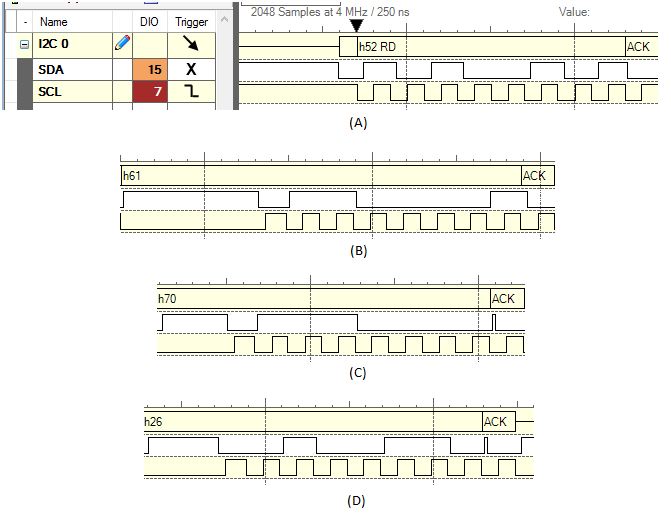
\includegraphics[width=\textwidth]{Test/images/readvaluesEdited.png}
	\caption{Tidslinje af aflæste I2C beskeder af PSoC0 fra Wii-Nunchuck}
	\label{fig:NunchuckReadValues}
\end{figure}

\begin{figure}[H]
	\centering
	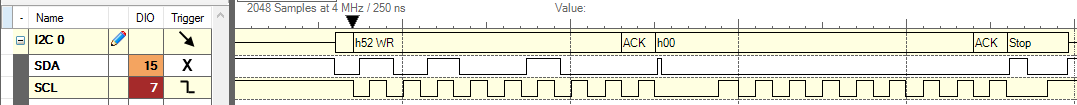
\includegraphics[width=\textwidth]{Test/images/writerequest}
	\caption{}
	\label{fig:NunchuckWriteValues}
\end{figure}

\subsubsection{I2C Protokol}

\subsection{Hardware}

\section{Integration}

\section{Accepttest}